% *** DOCUMENT CLASS ***%
\documentclass[11pt,compress]{beamer} % handout,
\usetheme{Madrid}
\usecolortheme{crane}
\useoutertheme[subsection=false,shadow]{miniframes}

% ! full class documentation available here
% http://tug.ctan.org/macros/latex/contrib/beamer/doc/beameruserguide.pdf

%===============================================
% *** GENERAL PACKAGES *** %
\usepackage[utf8]{inputenc}
\usepackage[english]{babel}
\usepackage{csquotes}
\usepackage{array}
\usepackage{booktabs}
\usepackage{multirow}
\usepackage{color}
\usepackage{lipsum}

%===============================================
% *** ALGORITHM PACKAGE *** %
\usepackage[ruled,vlined]{algorithm2e}
\newcommand{\forcond}[2]{#1 \KwTo #2}
\SetAlgoSkip{}

%===============================================
% *** GRAPHICS RELATED PACKAGES *** %
\usepackage{graphicx}
\DeclareGraphicsExtensions{.pdf,.jpg,.png,.gif}
\graphicspath{img}

%===============================================
% *** MATH PACKAGES *** %
\usepackage{amsfonts}
\usepackage{amsmath}
\usepackage{amsthm}
\usepackage{amssymb}
\usepackage{mathrsfs} % Ralph Smith’s Formal Script Font : mathrsfs{A}
\usepackage{mathtools}
\usepackage{siunitx}  % physics units
\usepackage{bm}
\usepackage{stmaryrd}

%===============================================
% *** BIBLIOGRAPHY PACKAGE *** 
\usepackage[backend=biber, style=authortitle]{biblatex}
\addbibresource{_report.bib}
\usepackage{appendixnumberbeamer}

% display table of content at the beginning of each section
\AtBeginSection[] {
    \ifnum \value{section}=1
      {
      \begin{frame}
        \frametitle{Overview}
          \small \tableofcontents[sectionstyle=show/shaded]
      \end{frame}
      }
    \else{
      \begin{frame}
          \small \tableofcontents[currentsection,sectionstyle=show/shaded,hideothersubsections]
      \end{frame}}
    \fi
    }
   \setbeamertemplate{caption}[numbered]
   
   \newcommand\blfootnote[1]{%
    \begingroup
    \renewcommand\thefootnote{}\footnote[frame]{#1}%
    \addtocounter{footnote}{-1}%
    \endgroup
   }

\begin{document}

\title[]{Detection of AI-generated images}
\author{Lucas SALAND\\ Supervisor: Patrick Bas}
\institute{Université de Lille}
\date[\today]{\includegraphics[keepaspectratio,width=0.2\textwidth]{img/cristal.png} \medskip \\ Lille, France \medskip \\ \today}

\frame{\titlepage}

\section*{Overview}
\begin{frame}
  \tableofcontents
\end{frame}

\section{AI image generation}
\subsection{GAN}
\subsection{Diffusion model}

\section{AI-generated images detection}
\subsection{CLIP}
\begin{frame}
    \frametitle{CLIP}
    \begin{figure}
        \includegraphics[width=\textwidth]{img/CLIP.png}
    \end{figure}
\end{frame}

\begin{frame}
  \frametitle{CLIP for detection}
  \only<1-4>{
    Method proposed in \autocite*{cozzolinoRaisingBarAIgenerated2024}:
  \begin{itemize}
    \pause
    \item Build a dataset of pairs of real and generated images
    \pause
    \item Extract the CLIP features
    \pause
    \item Train a SVM on these features
  \end{itemize}}
\end{frame}

\begin{frame}
  \frametitle{ELSA dataset}
  \begin{figure}
    \includegraphics[width=\textwidth]{img/ELSA.png}
  \end{figure}

\end{frame}

\subsection{Impact of JPEG compression}
\begin{frame}
    \frametitle{JPEG compression's impact}
    \only<1>{
    \begin{figure}
        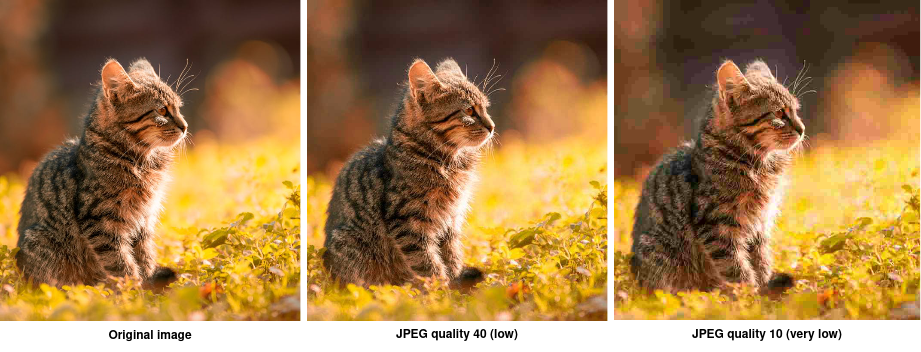
\includegraphics[width=\textwidth]{img/jpeg.png}
    \end{figure}
    }
    \only<2>{
    \begin{table}[H]
        \centering
        \begin{tabular}{|c|c|c|c|c|}
        \hline
        & \multicolumn{4}{c|}{Test} \\
        \cline{2-5}
         & quality & 40 & 65 & 90 \\
        \hline
        \multirow{3}{*}{Train} & 40 & 0.9813 & 0.9730 & 0.9797 \\
         \cline{2-5}
         & 65 & 0.9450 & 0.9825 & 0.9830 \\
         \cline{2-5}
         & 90 & 0.7744 & 0.8581 & 0.9925 \\
        \hline
        \end{tabular}
        \caption{Accuracy of binary classification for pairs of qualtity factors for train and test.}
        \label{table:jpeg}
    \end{table}
    }
\end{frame}


\subsection{Generators diversity and neural network}
\begin{frame}{Generators diversity and neural network}
  \begin{columns}
    \begin{column}{.4\textwidth}
      Synthbuster:
      \begin{itemize}
        \item 9 generators
        \item 1000 images per generator
      \end{itemize}
    \end{column}

    \begin{column}{.6\textwidth}
      \begin{figure}
        \includegraphics[width=\textwidth]{img/confusion.png}
        \caption{Confusion matrix for a SVM multiclass-classifier trained and tested on synth-
        buster.}
      \end{figure}
    \end{column}
  \end{columns}
\end{frame}

\begin{frame}{Generators diversity and neural network}
  Multi-class classifier for binary classification:
  \begin{figure}
    \includegraphics[width=\textwidth]{img/maps.png}
  \end{figure}
\end{frame}

\subsection{Pair training and fine-tuning}

\subsection{DoubleCLIP: Another approach to work with pairs}

\subsection{Tip-Adapter}

\section{Conclusion}
\end{document}